\documentclass{article}
\usepackage[spanish]{babel}%Configuracion en español
\usepackage[utf8]{inputenc}%Permite caracteres con tildes y ñ
\usepackage{graphicx}%Incluir imagenes
\usepackage{caption}
\usepackage{subcaption}%Subfiguras
\usepackage[table,xcdraw]{xcolor}%Color a tablas
\usepackage{biblatex}
\usepackage{amsmath, amssymb, amsthm}
\usepackage{enumitem}
\usepackage{tocloft}
\addbibresource{bibliografia.bib}

\title{Mi primer documento de primeros pasos en LaTex}
\author{David Alejandro Hrtado Palma}
\date{Octubre 2024}

\begin{document}
\maketitle

\newpage
\tableofcontents
\listoffigures
\listoftables
\newpage

\section{Introducción}
El presente docuemtno ilustar de forma practica las principales caracteristicas al momento de escribir con Latex.

\section{Generalidades}

\subsection{Niveles de los titulos}

En Latex se puede organizar la información por titulos hasta de tercer nivel utilizando los comandos\\

\setlength{\parindent}{2em} % Ajusta el tamaño de la sangría aquí

Mediante el comando \textbf{\textbackslash section\{\}} se emanrca el titulo de nivel 1. \\

Mediante el comando \textbf{\textbackslash subsection\{\}} se emanrca el titulo de nivel 2. \\

Mediante el comando \textbf{\textbackslash subsubsection\{\}} se emanrca el titulo de nivel 3.\\

\noindent Estos fueron los principales niveles de titulos en Latex. Esta sección ilustra como se puede aplicar una
sangria a una parte del texto y luego volver a sangrado normal


\subsubsection{Ejemplo de titulo de 3 nivel}

Este apartado muestra un ejemplo de incluir un titulo de nivel 3

\subsection{Paragrafos}

\paragraph{Ejemplo de paragrafo} 
Este es un ejemplo de paragrafo

\subparagraph{Ejemplo de paragrafo de segundo nivel} 
Por medio del comando utilizado se puede incluir un paragrafo de segundo nivel

\section{Listas}
Para el caso de las listas, estas se pueden clasificar en tres:

\begin{enumerate}
	\item Listas enumeradas
	\item Listas de items no enumeradas
	\item Listas combinadas

\end{enumerate}

\subsection{Listas enumeradas}
Para el caso de listas enumeradas originalmente viene para que fueran solo numericas e 1,2,3 ...
sin embargo utilizando el label \textbf{\textbackslash alph} puede crearce la lista de literales a, b, c

\subsubsection{Ejemplo lista numerales}

\begin{enumerate}
	\item Ejemplo 1
	\item Ejemplo 2
	\item Ejemplo 3

\end{enumerate}

\subsubsection{Ejemplo lista literales}

\begin{enumerate}[label=\alph*)]
	\item Ejemplo a
	\item Ejemplo b
	\item Ejemplo c
\end{enumerate}

\subsection{Lista de itens no numerados}

\begin{itemize}
	\item Manzana
	\item banano
	\item Pera
\end{itemize}

\subsection{Lista combinada}

A continuación se muestra una lista combinada de hasta tres niveles

\begin{enumerate}
	\item Comprar ingedientes
	\item Lavar ingrdientes
		\begin{enumerate}[label=\alph*)]
			\item Frutas
			\item Verduras
			\item Carnes
			\begin{itemize}
				\item Carnes rojas
				\item Carnes blancas
			\end{itemize}
			\item Utensilios empleados
		\end{enumerate}
	\item Preparar receta
		\begin{enumerate}[label=\alph*)]
			\

\end{enumerate}

\section{Figuras}

\subsection{Figuras simples}

Aca se presentan figuras simples

\begin{figure}[!h]

	\centering
	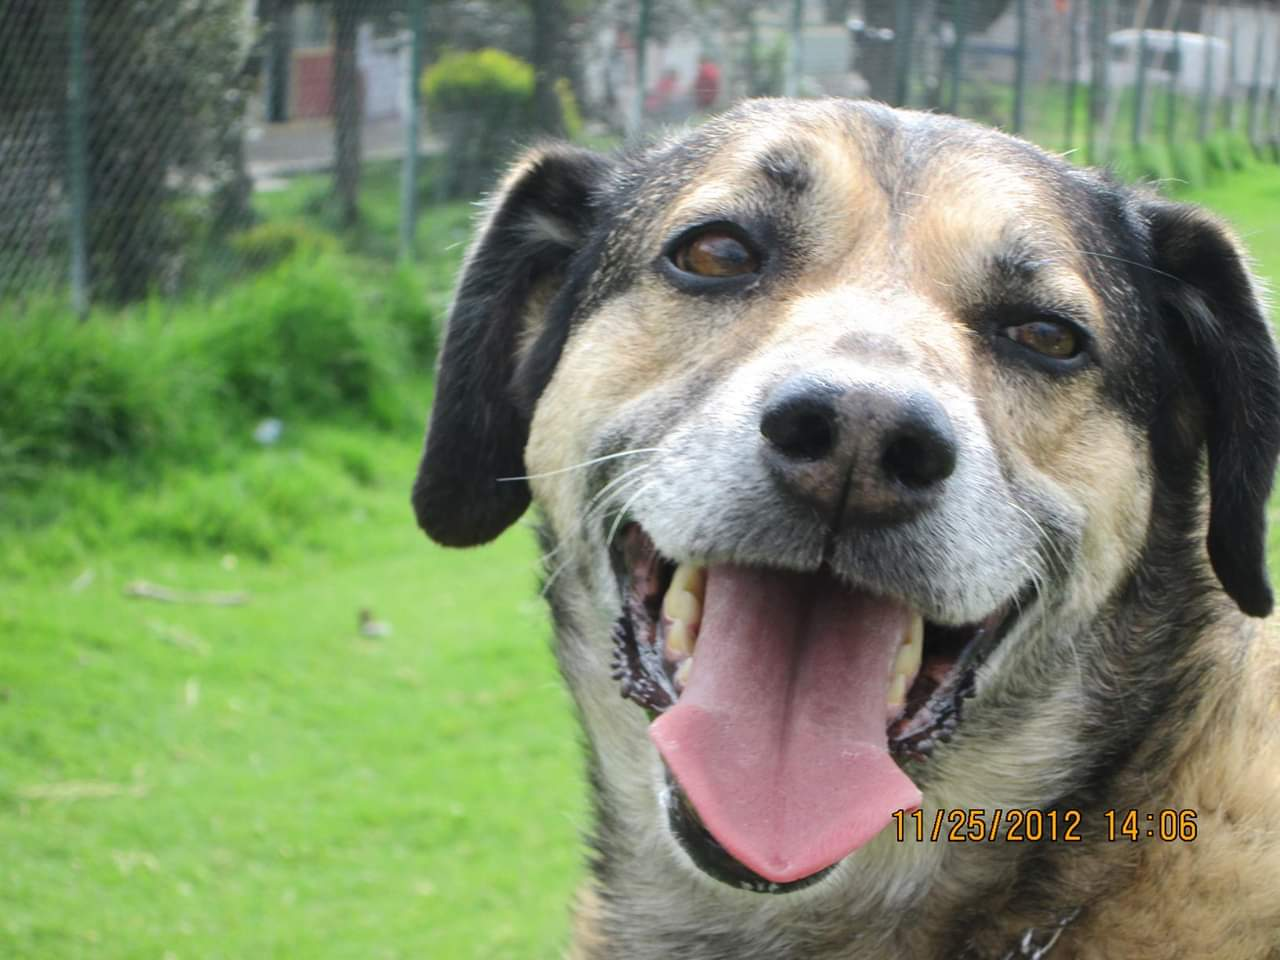
\includegraphics[width = 1\textwidth]{Imagenes/Pinina.jpg}
	\caption{Foto de Pinina en noviembre de 2012}
	\label{Pinina}
	
\end{figure}

\subsection{Figuras Compuestas}

\begin{figure}[h!]
	\begin{subfigure}{0.5\textwidth}
		\centering
		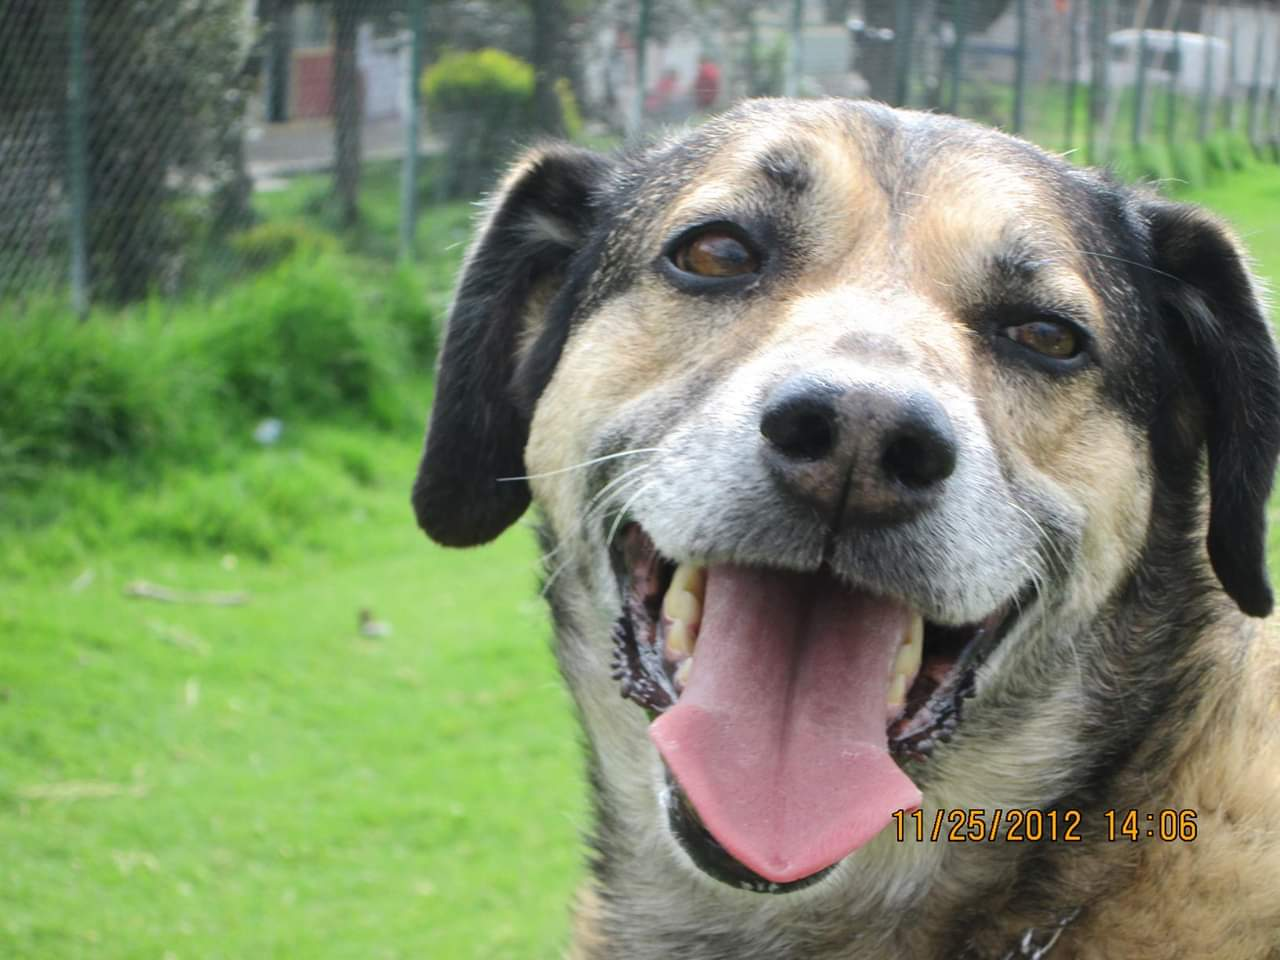
\includegraphics[width = 0.8\textwidth]{Imagenes/Pinina.jpg}
		\caption{Pinna}
		\label{Pinina2}		
	\end{subfigure}
	\begin{subfigure}{0.5\textwidth}
		\centering
		
\includegraphics[width = 0.8\textwidth]{Imagenes/Magis.JPG}
		\caption{Magis}
		\label{Magis}		
	\end{subfigure}
	\begin{subfigure}{0.5\textwidth}
		\centering
		
\includegraphics[width = 0.8\textwidth]{Imagenes/Homero.jpg}
		\caption{Homero y Snopy}
		\label{homeroSnoopy}		
	\end{subfigure}
	\begin{subfigure}{0.5\textwidth}
		\centering
		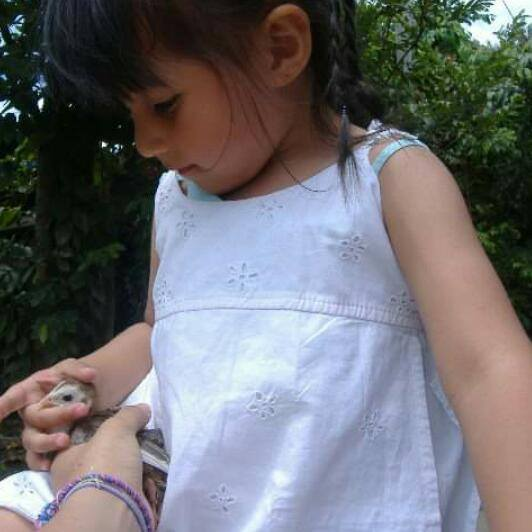
\includegraphics[width = 0.5\textwidth]{Imagenes/Sofia.jpg}
		\caption{Sofia}
		\label{Sofia}		
	\end{subfigure}

	\caption{Ejemplos images compuestas}
	\label{FiguraVarias}
	
\end{figure}

\newpage

\section{Tablas}

Para el caso de tablas debido a que escribir en texto plano el contenido de las tablas
puede ser un poco engorroso, se utiliza para esto la aplicación \textbf{Excel2LaTeX}, el cual es un complemento para
instalar en Excel \cite{TalasExcel}

\begin{table}[htbp]
	\centering
	\caption{Ejemplo de tabla}
	  \begin{tabular}{lllll}
	  Encabezado 1 & Encabezado 2 & Encabezado 3 & Encabezado 4 & Encabezado 5 \\
	  Dato 1 & Dato 2 & Dato 3 & Dato 4 & Dato 5 \\
	  Dato 6 & Dato 7 & Dato 8 & Dato 9 & Dato 10 \\
	  Dato 11 & Dato 12 & \cellcolor[rgb]{ 1,  1,  0}Dato 13 & Dato 14 & Dato 15 \\
	  Dato 16 & Dato 17 & Dato 18 & Dato 19 & Dato 20 \\
	  \end{tabular}%
	\label{PrimerTablaEjemplo}%
  \end{table}%

\newpage

\section{Citas bibliograficas}

En la figura o  imagen \ref{Pinina} e imagen \ref{Pinina2} como en la se puede ver a mi perrita Pinina \footnote{Ese nombre no se lo pusimos nosotros, ya venia asi}\\

Para las citas bibliograficas fue utilizada la informacion de paperpile \cite{CitasBiliografica}


\section{Ecuaciones}

\subsection{Ecuaciones simples sobre linea}

Para una ecuación definida dentro de una linea $a^2 + b ^2 = c^2 $ se realiza con un solo signo de peso ( \$ )

\subsection{Ecuaciones en linea diferente}
Otro ejemplo deecuación es: $$a/b = c/b'$$

\subsection{Ecuaciones numeradsa}

\begin{equation}
	x^3 + 2x^2 = 3
\end{equation}


\begin{equation}
	\sqrt{x} + 2x^2 = 3
\end{equation}

\begin{equation}
	a^2 + b ^2 = c^2
	\label{EcPitagoras}
\end{equation}

\begin{equation}
	\int_{a}^{b} f(x)dx = F(b) - F(a)
	\label{Integral1}
\end{equation}


Para citar una ecuacion se utiliza el mismo mecanismo para citar las tablas. 
Por ejemplo para señalar la ecuación de pitagoras que corresponde a la ecuación  \ref{EcPitagoras}

La ecuación npumero \ref{Integral1} fue tomada como ejemplo de \cite{EcuacionesMath}


\section{Template o plantillas}

En la pagina de Overleaf \cite{PlantillasOverlaf} es posible revisar diferentes platillas para diversos usos

\printbibliography

\end{document}